\documentclass{article}
\usepackage{graphicx}
\usepackage{siunitx}
\graphicspath{ {images/} }
\title{Cart Rolling Down Ramp}
\author{Grant Curell}
\begin{document}
\maketitle{}
\section{Problem}
Here, a cart is about to roll down a ramp. The cart travels not only vertically but also horizontally along the ramp, which is inclined at an angle $\theta$. Say that $\theta$ = \ang{30} and that the length of the ramp is 5.0 meters. How fast will the cart be going at the bottom of the ramp?

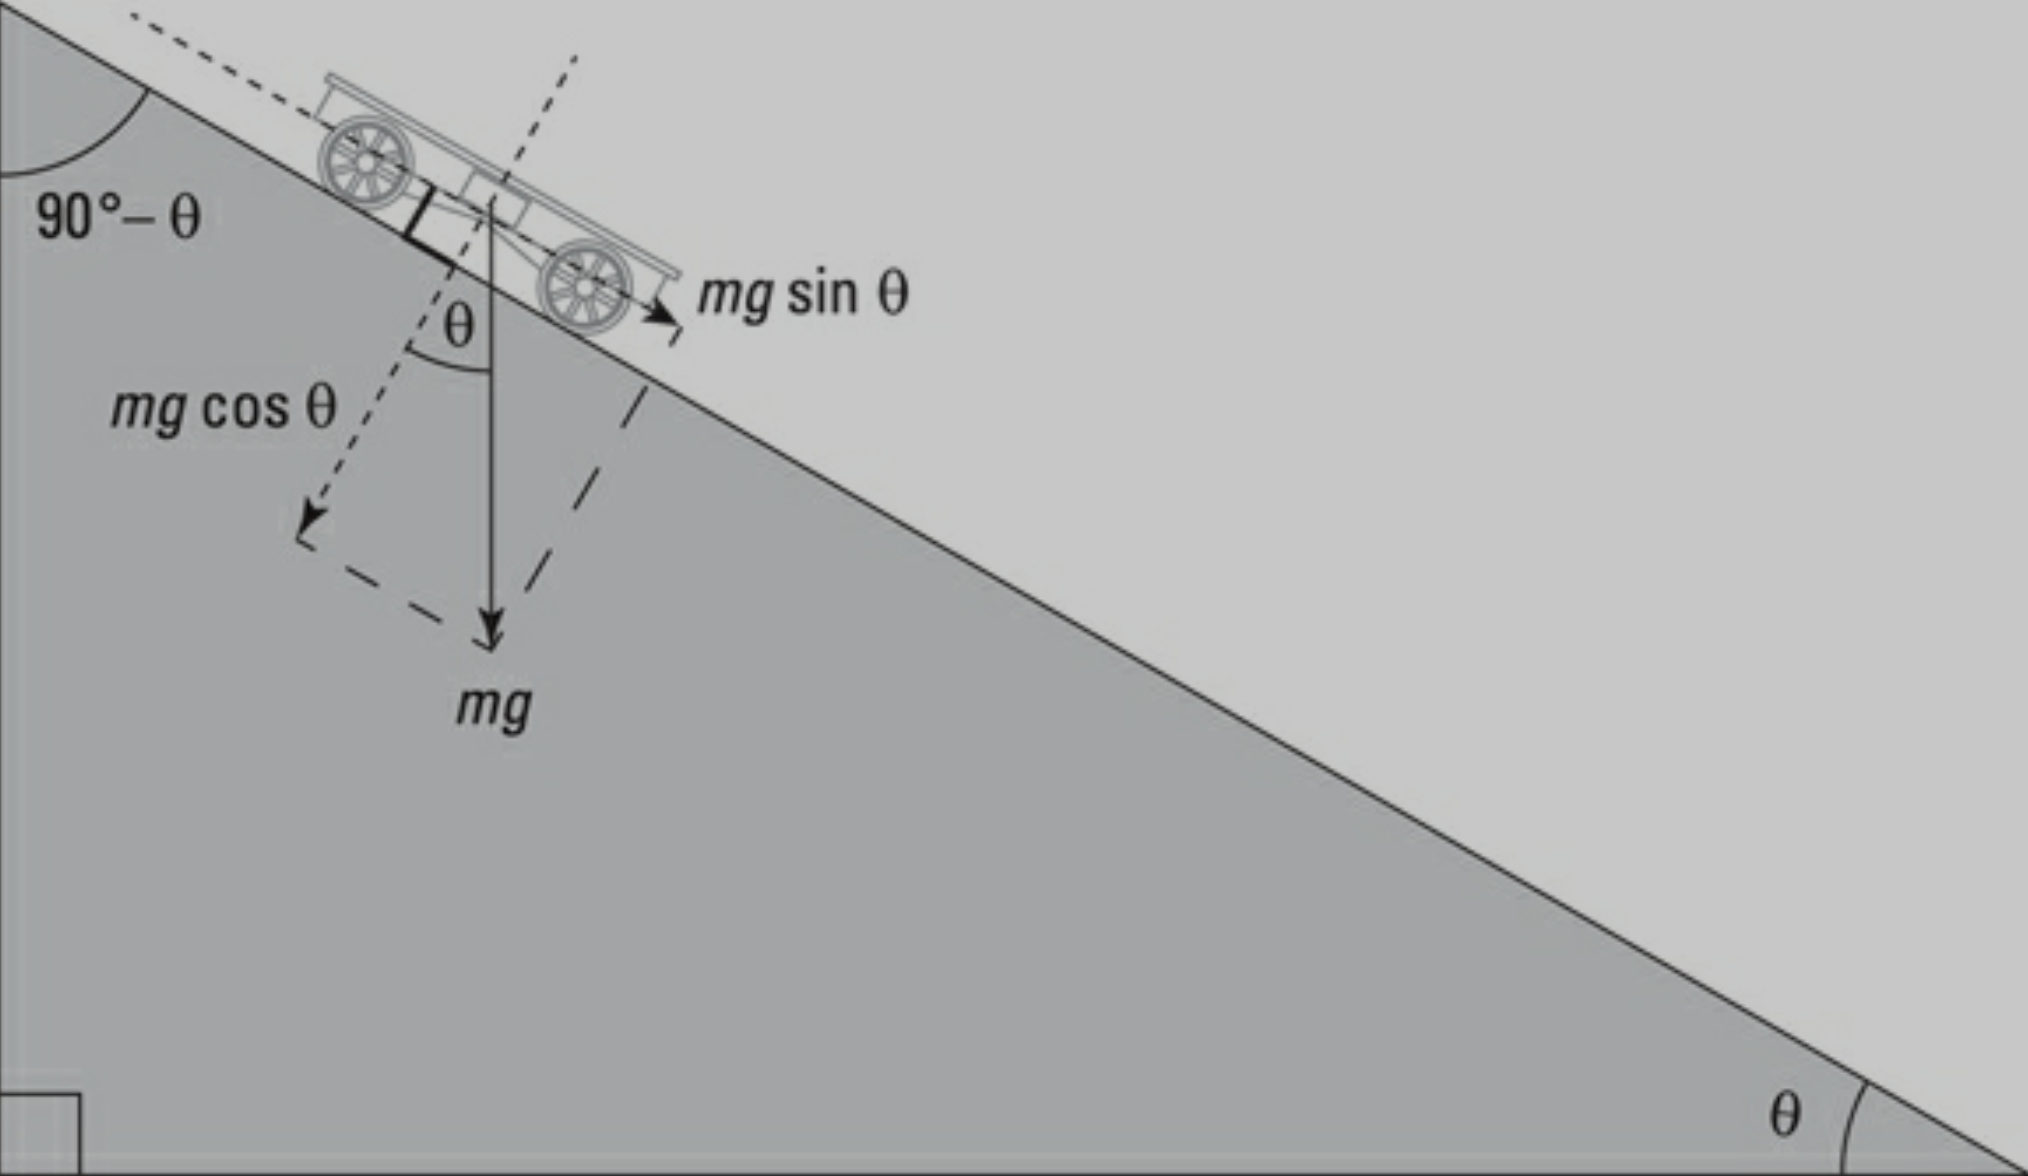
\includegraphics[width=\columnwidth]{image}
\\\\
Holzner, Steven. Physics I For Dummies (For Dummies (Math \& Science)) (pp. 100-101). Wiley. Kindle Edition.
\\\\
\section{Solution}
\[ \theta=\ang{30} \]
\[ s=5m \]
\[ mg\sin(30)=F_{ramp} \]
\[ F_{ramp}=ma \]
\[ ma=mg\sin(\theta) \]
\[ a=g\sin(\theta) \]
\[ a=g\sin(\theta)=\frac{v_f}{t} \]
\[ s=\frac{v_ft}{2} \]
\[ 5=\frac{v_ft}{2} \]
\[ \frac{10}{v_f}=t \]
Taking from the equation we derived in the above.
\[ g\sin(\theta)=\frac{v_f}{t} \]
\[ 9.8\sin(30)=\frac{v_f^2}{10} \]
\[ v_f=7.0m/s \]
\end{document}
